\documentclass[border=10pt]{standalone}

\usepackage{tikz}
\usepackage{tikzsymbols}
\usetikzlibrary{calc,patterns,shapes.geometric}

\def\centerarc[#1](#2)(#3:#4:#5){\draw[#1] ($(#2)+({#5*cos(#3)},{#5*sin(#3)})$) arc (#3:#4:#5);}

\begin{document}
	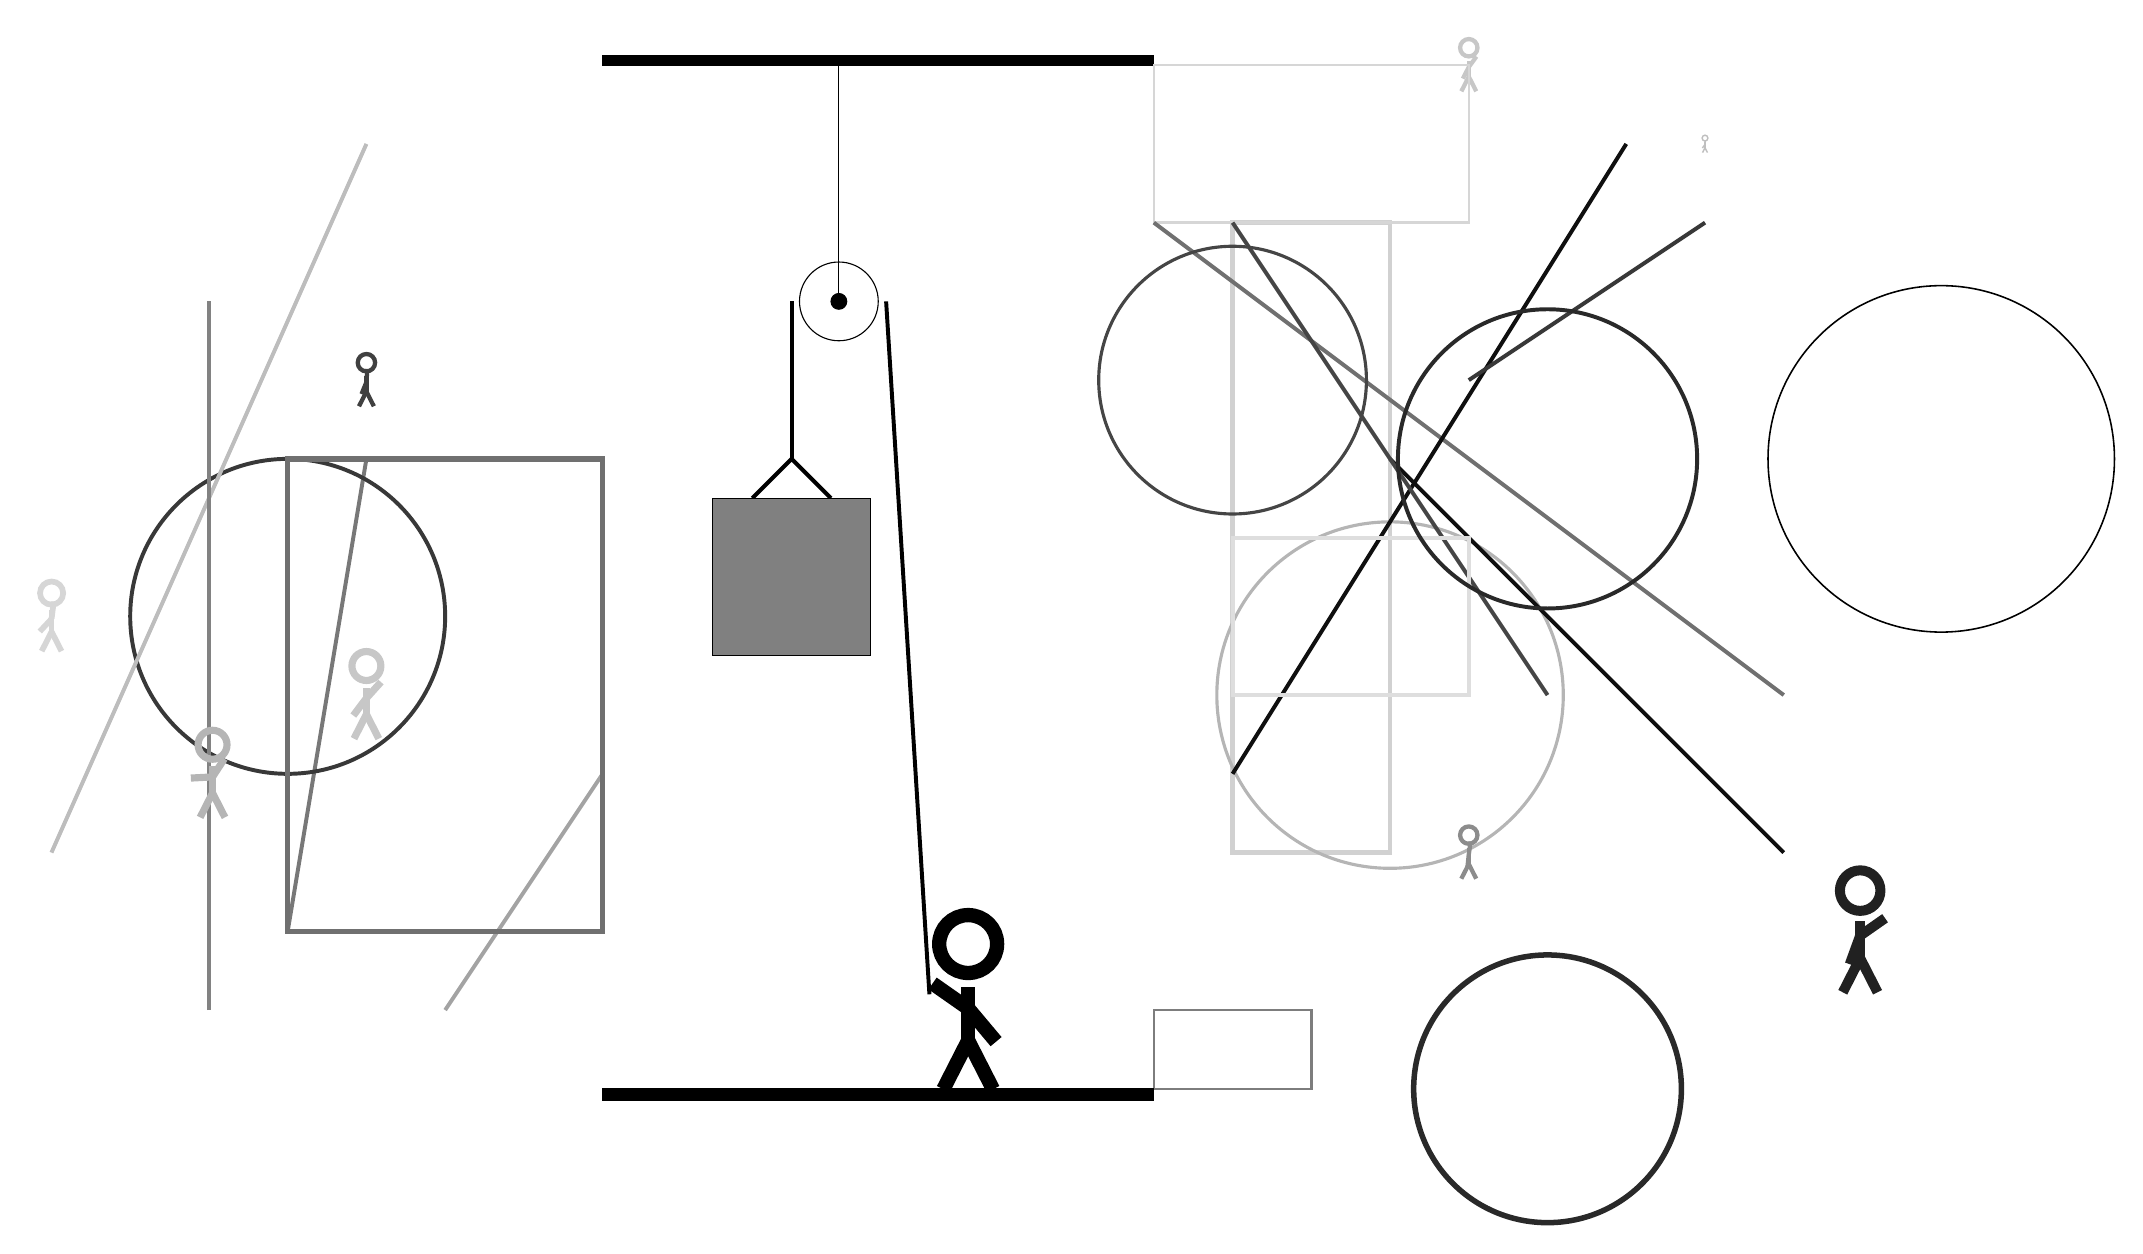
\begin{tikzpicture}
		%%%%% START %%%%%
		
		\draw[fill=black] (-2, 10) rectangle (5, 10.125);
		
		\draw (1, 7) circle (0.5);
		\draw[fill=black] (1, 7) circle (0.1);
		\draw (1, 10) -- (1, 7);
		
		\draw[line width=0.5mm] (-0.1, 4.5) -- (0.4, 5.0) -- (0.9, 4.5);
		\draw[fill=black!50] (-0.6, 4.5) rectangle (1.4, 2.5);
		
		\draw[line width=0.5mm] (0.4, 7) -- (0.4, 5.0);
		\centerarc[line width=0.5mm](1, 7)(0:180:0.6);
		\draw[line width=0.5mm](1.6, 7) -- (2.15, -1.8);
		
		\node[line width=0.4mm, color=black!25] at (12, 9) {\Strichmaxerl[1][52][88]};
		
		\draw[line width=0.6mm, color=black!18] (6, 0) rectangle (8, 8);
		\draw [line width=0.4mm, color=black!29](8, 2) circle (2.2);
		\node[line width=0.6mm, color=black!22] at (9, 10) {\Strichmaxerl[3][63][54]};
		
		\node[line width=0.4mm, color=black!87] at (14, -1) {\Strichmaxerl[7][70][35]};
		\draw[line width=0.5mm, color=black!53](-6, -1) -- (-5, 5);
		\draw[line width=0.3mm, color=black!16] (5, 10) rectangle (9, 8);
		
		\node[line width=0.6mm, color=black!16] at (-9, 3) {\Strichmaxerl[4][47][83]};
		\draw[line width=0.5mm, color=black!56](5, 8) -- (13, 2);
		
		\draw [line width=0.4mm, color=black!73](6, 6) circle (1.7);
		
		\draw [line width=0.5mm, color=black!78](-6, 3) circle (2.0);
		\draw [line width=0.7mm, color=black!84](10, -3) circle (1.7);
		\draw[line width=0.5mm, color=black!26](-5, 9) -- (-9, 0);
		
		\draw[line width=0.5mm, color=black!49](-7, -2) -- (-7, 7);
		\node[line width=0.6mm, color=black!75] at (-5, 6) {\Strichmaxerl[3][68][86]};
		\draw[line width=0.5mm, color=black!94](6, 1) -- (11, 9);
		
		\draw[line width=0.5mm, color=black!36](-2, 1) -- (-4, -2);
		\draw[line width=0.5mm, color=black!94](8, 5) -- (13, 0);
		\draw [line width=0.2mm, color=black!100](15, 5) circle (2.2);
		
		\draw[line width=0.5mm, color=black!73](10, 2) -- (6, 8);
		\draw[line width=0.5mm, color=black!13] (6, 2) rectangle (9, 4);
		
		\draw[line width=0.3mm, color=black!51] (7, -2) rectangle (5, -3);
		\draw[line width=0.7mm, color=black!56] (-2, 5) rectangle (-6, -1);
		\draw[line width=0.5mm, color=black!78](9, 6) -- (12, 8);
		\node[line width=0.2mm, color=black!22] at (-5, 2) {\Strichmaxerl[5][53][48]};
		\node[line width=0.4mm, color=black!29] at (-7, 1) {\Strichmaxerl[5][3][57]};
		\node[line width=0.4mm, color=black!45] at (9, 0) {\Strichmaxerl[3][84][82]};
		\draw [line width=0.5mm, color=black!84](10, 5) circle (1.9);
		
		\node at (2.6, -1.9) {\Strichmaxerl[10][-35][-50]};
		
		\draw[fill=black] (-2, -3) rectangle (5, -3.15);
		
		%%%%% END %%%%%
	\end{tikzpicture}
\end{document}